\section{Discussion and Limitations}
\label{sec:discussion}

The main value of CodeGraph is not only that it improves retrieval accuracy, but that its failure modes are structurally interpretable. Because ranking is deterministic and graph-constrained, missed targets can be traced to missing reachability rather than opaque model behavior. This makes the remaining limitations scientifically informative, and also suggests where hybrid retrieval systems should focus future effort.

\subsection{Practical Implications for AI Coding Agents}

For AI coding agents to operate autonomously, they require retrieval tools that are not only accurate but stable. When an agent requests context, it needs a fast, predictable response. Systems that place large language models directly inside the retrieval loop (e.g., to generate graph queries or re-rank snippets) introduce high latency and non-deterministic variance. An agent debugging a failure may receive a different context window upon retrying the exact same task.

CodeGraph provides a deterministic foundation for agent memory. By separating the graph construction (performed asynchronously) from the ranking phase (performed via deterministic matrix multiplication), the system guarantees that the same seed set will always produce the exact same topological ranking. This allows agent designers to cache results, write reproducible evaluation harnesses, and treat the repository graph as a stable environment rather than a stochastic oracle.

\subsection{Structural Limitations and Future Hybridization}

An analysis of the zero-recall instances defines the exact boundaries of static graph-based retrieval. We identify two primary failure modes (\Cref{fig:taxonomy}):

\begin{figure}[htbp]
    \centering
    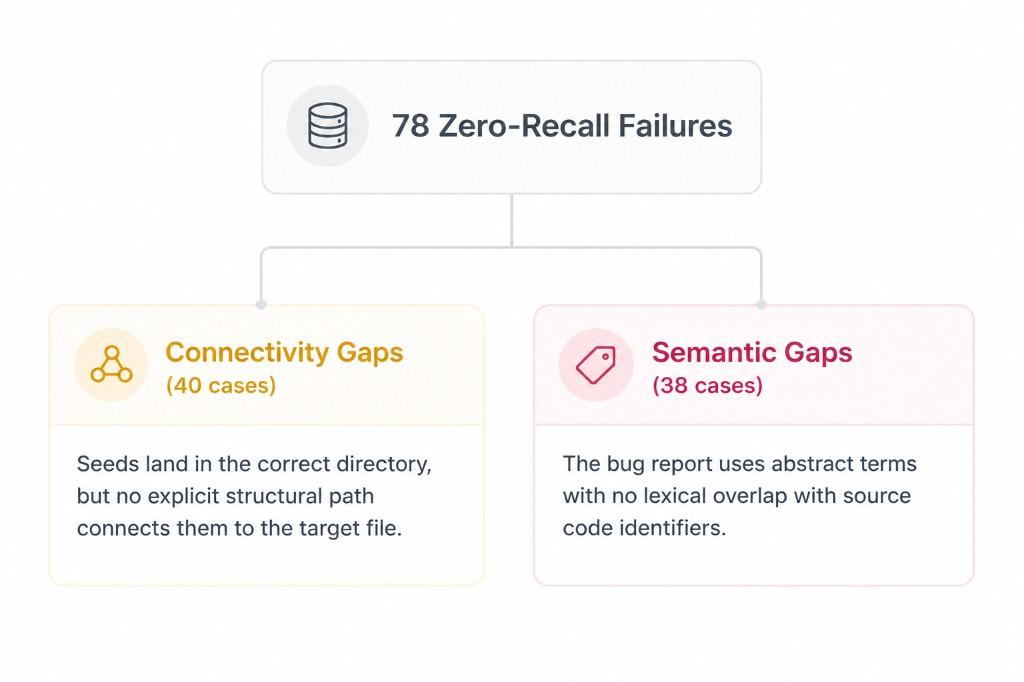
\includegraphics[width=\linewidth]{assets/failure_taxonomy.png}
    \caption{Failure taxonomy of the zero-recall instances. Connectivity Gaps account for 40 cases (missing graph edges), and Semantic Gaps account for 38 cases (lexical mismatch).}
    \label{fig:taxonomy}
\end{figure}

\textbf{Connectivity Gaps (40 instances):} These occur when seeds land in the correct general region, but no explicit syntactic dependency (e.g., \texttt{CALLS} or \texttt{IMPORTS}) connects the seed to the specific target file. Files that collaborate through implicit data flows, configuration files, or dynamic plugin registries remain invisible to standard structural propagation. This establishes the ceiling of purely static graph retrieval.

\textbf{Semantic Gaps (38 instances):} These failures arise when the issue description uses highly abstract natural-language terms with zero lexical overlap with any source-code identifier. Without a lexical anchor, the system cannot place any seed in the relevant neighbourhood, causing a total reachability failure.

These limitations naturally motivate the next stage of hybridization. To bridge semantic gaps without sacrificing determinism, future systems should investigate employing lightweight dense embeddings strictly for the initial seed selection stage, allowing abstract tasks to anchor correctly before delegating the final ranking back to the graph structure. To bridge connectivity gaps, integrating dynamic execution traces or semantic data-flow edges could expose implicit dependencies that static syntax misses, yielding an even more complete topological view of the repository.
